%\title{SWEETcam submission for IEEE Computer}

%%
%% Draft version 1.0
%%
%% Authors:
%% Kevin Abas
%% Caio Porto
%% Katia Obraczka 
%%

%% The template used was by Michael Shell
%% see http://www.michaelshell.org/
%% for current contact information.

%%*************************************************************************
%% Legal Notice:
%% This code is offered as-is without any warranty either expressed or
%% implied; without even the implied warranty of MERCHANTABILITY or
%% FITNESS FOR A PARTICULAR PURPOSE! 
%% User assumes all risk.
%% In no event shall IEEE or any contributor to this code be liable for
%% any damages or losses, including, but not limited to, incidental,
%% consequential, or any other damages, resulting from the use or misuse
%% of any information contained here.

%%*************************************************************************

\documentclass[journal,transmag]{IEEEtran}

% *** GRAPHICS RELATED PACKAGES ***
%
\usepackage{graphicx}
\ifCLASSINFOpdf

\else

\fi

% *** ALIGNMENT PACKAGES ***
%
\usepackage{array}

% *** PDF, URL AND HYPERLINK PACKAGES ***
%
\usepackage{url}
% url.sty was written by Donald Arseneau. It provides better support for
% handling and breaking URLs. url.sty is already installed on most LaTeX
% systems. The latest version and documentation can be obtained at:
% http://www.ctan.org/tex-archive/macros/latex/contrib/url/
% Basically, \url{my_url_here}.

% correct bad hyphenation here
\hyphenation{op-tical net-works semi-conduc-tor}

% ** BIBTEXT PACKAGE **
\usepackage{cite}


%%----------------------------------------------------------------------

\begin{document}


%% ***********************  THE TITLE **********************************

\title{Designing Efficient Smart Camera Networks For Public Saftey}


%% ***********************  AUTHORS ************************************

\author{\IEEEauthorblockN{Kevin Abas\IEEEauthorrefmark{1},
Caio Porto\IEEEauthorrefmark{2},
Katia Obraczka\IEEEauthorrefmark{1}}
\IEEEauthorblockA{\IEEEauthorrefmark{1}School of Engineering,
University of California Santa Cruz, CA 95064 USA}
\IEEEauthorblockA{\IEEEauthorrefmark{2}Escola Politecnica ´
Avenida Athos da Silveira Ramos ´
Rio de Janeiro, 21941-909, Brazil}
}


%% ***********************  AUTHORS ************************************

\IEEEtitleabstractindextext{%
\begin{abstract}
The abstract goes here.
\end{abstract}


%% ********************** IEEE KEYWORDS ********************************

\begin{IEEEkeywords}
IEEEtran, journal, \LaTeX, magnetics, paper, template.
\end{IEEEkeywords}}



%% Title Configurations (From Template)
\maketitle
\IEEEdisplaynontitleabstractindextext
\IEEEpeerreviewmaketitle


%% *********************  BEGIN PAPER **********************************

\section{Introduction}


\IEEEPARstart{T}{his} paper discusses ...

\subsection{Background, motivation} 
\-- Goals of the paper, What problems this papers solves \\

\subsubsection{Today's applications (summary)}
\-- Some things current Smart Camera networks assist with when it comes to 
surveillance and crime detection nodes. \\

%%Requirements for today's wireless Smart Camera Networks

\section{Smart Camera Surveillance}
Researchers and Commercial companies are designing wireless smart camera networks in surveillance applications to prevent crimes in public spaces. To
understand how these state of the art systems are improving on designs of the past one must define what makes these surveillance systems "smart". These
smart camera network systems have common goals when it comes creating more efficient surveillance applications. First, the issue of network resource
utilization is an issue all systems need to consider if those surveillance systems are to be scalable in crowded wireless deployment scenarios. Then in
almost every application considering power consumption of each node is very important if one is give an analysis of the systems efficiency. If these
systems are to be monitoring public spaces the smart camera networks need to be keeping the data recorded secure and also ensuring that the data recorded
is actually quality information that could be used by officials. \\


%% Wireless Smart Camera Networks Taxonomy Divided into 3 sections
%% 1 Bandwidth efficieny 2 power consumption 3 Quality of data
\subsection{Bandwidth Efficiency}
Video data is rich with useful information that other sensor source can’t provide, however video data quickly becomes very large in size as time goes on.
Nodes competing for network connectivity while maintaining quality on live video feed can soon become a problem as the network grows or if other nodes
not in the system share the connection. One way to combat this is by assuring the data recorded is useful and actually recording video data that can be
used to do detection of events. A common technique is to use other non-image sensors to provide separate data that can be used to determine if the camera
should record video at all.

\-- A comparison chart of different hardware components of their systems 
	being used\\ \\
\-- A comparison chart of software design features (computer vision, network
	topologies, bandwidth/energy saving techniques, etc. )\\ \\
\-- Explain each classification criterion, provide examples, etc.\\ \\

\subsection{Lowering Power Consumption}

\subsection{Quality of data produced}

\section{Example Wireless Smart Camera Systems}
\-- Going into more detail of possibly one of the examples shown above in
	the taxonomy\\ \\
\--

\section{Our Project}

\subsection{Hardware}
 \-- Discuss breifly about the different components and why they were chosen \\

\subsubsection{WiFi 802.11n \\}
\subsubsection{MSP430 \\}

\subsection{Software}
\subsubsection{Image Processing}
\- Considering the constraints of the system in terms of price and hardware, it is used techniques of background subtraction to do the object detection. When started, the program keep taking pictures and process them using Mixture of Gaussian (MoG) method by Stauffer and Grimson. With the foreground in hands we find the contours and then a bounded box is applied following the contours' limit. To remove some noise and false detection a step is added to ignore objects of small size. The object classification is the most processor consumption  processes for most of the pedestrian detection systems, because it is used training techniques to classify the objects based on a previous stored database. In our case, to reduce the process we classify the objects by looking at their dimensions, they are classified as human if the height is two times bigger than the width we classify as a person. \\
\begin{figure}[h!]
\centering
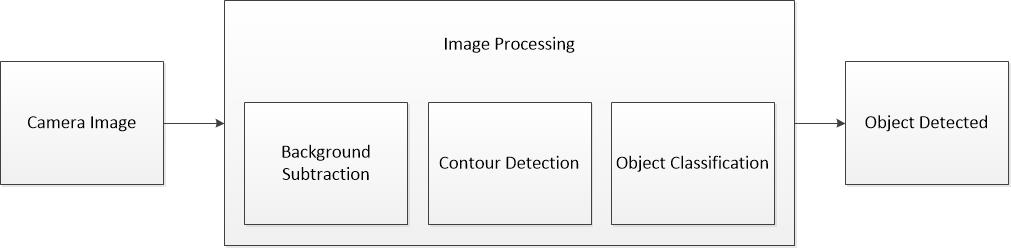
\includegraphics[scale=0.3]{imageprocessing.jpg}
\end{figure}	
\- This light system can generate some false alarms, but in association with the whole system, and its sensors, it can be improved for a better performance. There are other more robust object detection methods that could be used, but we would have a very low fps rate. \\
\- We developed using the Raspberry Pi camera module, which has already an API in C language and capable of capturing 1920x1080 resolution color images with 30 fps rate. For the image processing, we chose the Open Source Computer Vision Library (OpenCv). Our computer vision system is developed in C++ for better integration between the OpenCV and the API.\\

\subsection{Future Goals}

\section{Future Directions for Smart Wireless Camera Networks}
\-- Discuss research that has been proposed in the area and that is just begining to be implemented or hasn't yet at all.\\

\section{Lessons to take away}

\-- just so it compiles here are the references to be used:
~\cite{DSPcam}
~\cite{HuSIMS}
~\cite{Citric}
~\cite{OmniEye}
~\cite{ScoutNode}
~\cite{SensEye}
~\cite{WiFLIP}

%% *************************  END PAPER **********************************


% Can use something like this to put references on a page
% by themselves when using endfloat and the captionsoff option.
%\ifCLASSOPTIONcaptionsoff
%  \newpage
%\fi


%% ******************  REFERENCE SECTION **********************************

\bibliography{Bib.bib}{}
\bibliographystyle{plain}


%% ******************  AUTHOR BIOGRAPHIES *********************************

\begin{IEEEbiographynophoto}{Kevin Abas}
Biography text here.
\end{IEEEbiographynophoto}

\begin{IEEEbiographynophoto}{Caio Porto}
Biography text here.
\end{IEEEbiographynophoto}


\end{document}

%%------------------------------------------------------------------------



% *** MATH PACKAGES ***
%
%\usepackage[cmex10]{amsmath}
% A popular package from the American Mathematical Society that provides
% many useful and powerful commands for dealing with mathematics. If using
% it, be sure to load this package with the cmex10 option to ensure that
% only type 1 fonts will utilized at all point sizes. Without this option,
% it is possible that some math symbols, particularly those within
% footnotes, will be rendered in bitmap form which will result in a
% document that can not be IEEE Xplore compliant!
%
% Also, note that the amsmath package sets \interdisplaylinepenalty to 10000
% thus preventing page breaks from occurring within multiline equations. Use:
%\interdisplaylinepenalty=2500
% after loading amsmath to restore such page breaks as IEEEtran.cls normally
% does. amsmath.sty is already installed on most LaTeX systems. The latest
% version and documentation can be obtained at:
% http://www.ctan.org/tex-archive/macros/latex/required/amslatex/math/


% An example of a floating figure using the graphicx package.
% Note that \label must occur AFTER (or within) \caption.
% For figures, \caption should occur after the \includegraphics.
% Note that IEEEtran v1.7 and later has special internal code that
% is designed to preserve the operation of \label within \caption
% even when the captionsoff option is in effect. However, because
% of issues like this, it may be the safest practice to put all your
% \label just after \caption rather than within \caption{}.
%
% Reminder: the "draftcls" or "draftclsnofoot", not "draft", class
% option should be used if it is desired that the figures are to be
% displayed while in draft mode.
%
%\begin{figure}[!t]
%\centering
%\includegraphics[width=2.5in]{myfigure}
% where an .eps filename suffix will be assumed under latex, 
% and a .pdf suffix will be assumed for pdflatex; or what has been declared
% via \DeclareGraphicsExtensions.
%\caption{Simulation Results.}
%\label{fig_sim}
%\end{figure}

% Note that IEEE typically puts floats only at the top, even when this
% results in a large percentage of a column being occupied by floats.


% An example of a double column floating figure using two subfigures.
% (The subfig.sty package must be loaded for this to work.)
% The subfigure \label commands are set within each subfloat command,
% and the \label for the overall figure must come after \caption.
% \hfil is used as a separator to get equal spacing.
% Watch out that the combined width of all the subfigures on a 
% line do not exceed the text width or a line break will occur.
%
%\begin{figure*}[!t]
%\centering
%\subfloat[Case I]{\includegraphics[width=2.5in]{box}%
%\label{fig_first_case}}
%\hfil
%\subfloat[Case II]{\includegraphics[width=2.5in]{box}%
%\label{fig_second_case}}
%\caption{Simulation results.}
%\label{fig_sim}
%\end{figure*}
%
% Note that often IEEE papers with subfigures do not employ subfigure
% captions (using the optional argument to \subfloat[]), but instead will
% reference/describe all of them (a), (b), etc., within the main caption.


% An example of a floating table. Note that, for IEEE style tables, the 
% \caption command should come BEFORE the table. Table text will default to
% \footnotesize as IEEE normally uses this smaller font for tables.
% The \label must come after \caption as always.
%
%\begin{table}[!t]
%% increase table row spacing, adjust to taste
%\renewcommand{\arraystretch}{1.3}
% if using array.sty, it might be a good idea to tweak the value of
% \extrarowheight as needed to properly center the text within the cells
%\caption{An Example of a Table}
%\label{table_example}
%\centering
%% Some packages, such as MDW tools, offer better commands for making tables
%% than the plain LaTeX2e tabular which is used here.
%\begin{tabular}{|c||c|}
%\hline
%One & Two\\
%\hline
%Three & Four\\
%\hline
%\end{tabular}
%\end{table}


% Note that IEEE does not put floats in the very first column - or typically
% anywhere on the first page for that matter. Also, in-text middle ("here")
% positioning is not used. Most IEEE journals use top floats exclusively.
% Note that, LaTeX2e, unlike IEEE journals, places footnotes above bottom
% floats. This can be corrected via the \fnbelowfloat command of the
% stfloats package.


% if have a single appendix:
%\appendix[Proof of the Zonklar Equations]
% or
%\appendix  % for no appendix heading
% do not use \section anymore after \appendix, only \section*
% is possibly needed

% use appendices with more than one appendix
% then use \section to start each appendix
% you must declare a \section before using any
% \subsection or using \label (\appendices by itself
% starts a section numbered zero.)
%